\documentclass[11pt,fancychapters]{article}
\usepackage[a4paper, total={6in, 8in}]{geometry}
\usepackage{cite}
\usepackage{color}
\usepackage{xcolor}
\usepackage{empheq}
\usepackage{enumitem}
\usepackage{setspace}
\usepackage{hyperref}
\usepackage{minted}
\usepackage{acro}
\usepackage{amsmath}
\usepackage{amsthm}
\usepackage{amssymb}
\usepackage{multirow}
\usepackage{graphicx}
\usepackage{geometry}
\usepackage{subcaption}
\usepackage{cancel}
\usepackage[utf8]{inputenc}
\usepackage[english]{babel}
\usepackage{tcolorbox}
\usepackage{hyperref}
\usepackage{cleveref}
\usepackage{parskip}
\usepackage{tcolorbox}
\usepackage{float}
\usepackage{bm}
\usepackage{mathtools}
\usepackage{pgfplots}
 \geometry{
 a4paper,
 total={170mm,257mm},
 left=20mm,
 top=20mm,
 }
\pgfplotsset{width=8cm,compat=1.9}
\newcommand{\dbar}{{d\mkern-7mu\mathchar'26\mkern-2mu}}
\newcommand{\boxedeq}[2]{\begin{empheq}[box={\fboxsep=6pt\fbox}]{align}\label{#1}#2\end{empheq}}
\newcommand{\approptoinn}[2]{\mathrel{\vcenter{
  \offinterlineskip\halign{\hfil$##$\cr
    #1\propto\cr\noalign{\kern2pt}#1\sim\cr\noalign{\kern-2pt}}}}}
\newcommand{\appropto}{\mathpalette\approptoinn\relax}
\renewcommand*{\thesection}{\arabic{section}.}
\def\*#1{\mathbf{#1}}
\def\ab{ab}
\usepackage{tikz}
\usetikzlibrary{calc,trees,patterns,positioning,arrows,chains,shapes.geometric,%
    decorations.pathreplacing,decorations.pathmorphing,shapes,%
    matrix,shapes.symbols}
\usepgfplotslibrary{fillbetween}
\geometry{top=1.3in,bottom=1.3in}

\begin{document}
\centerline{\huge{SUTD 2021 50.007 Homework 3}}

\begin{table}[ht]
\centering
\footnotesize
 \begin{tabular}{c c} 
James Raphael Tiovalen & 1004555
 \end{tabular}
\end{table}

\section{Logistic Regression}

\subsection*{Question 1.1}

\begin{enumerate}[label=\textbf{\alph*)}]
	
\item True.

\item False. Despite the term ``regression" being present in the name of ``logistic regression", it is actually a classification algorithm. The term ``regression" is present simply because the output is a real number. However, the output is still bounded, and hence, it is solving a classification problem.

\item True. Logistic regression is a subset and a building block of neural network. Thus, a single-layer feedforward neural network (i.e., a single neuron with only one output) using the sigmoid activation function is equivalent to logistic regression.

\item False. The output probability value or confidence score is between 0 and 1, inclusive.

\end{enumerate}

\subsection*{Question 1.2}

The correct statements are:

\begin{enumerate}[label=\textbf{\arabic*)}]
	
\addtocounter{enumi}{1}
	
\item Our estimate for $P(y=0|x;\theta)$ is 0.72.

\item Our estimate for $P(y=1|x;\theta)$ is 0.28.
	
\end{enumerate}

This is because $h_\theta(x)$ is the estimated probability that $y = 1$ on input $x$. Hence, by this definition, it implies that $P(y=1|x;\theta) = 0.28$.

Additionally, since $P(y=0|x;\theta) + P(y=1|x;\theta) = 1$, we can substitute the value that we have previously to obtain $P(y=0|x;\theta) = 1 - 0.28 = 0.72$.

\subsection*{Question 1.3}

Given that $\theta = \begin{bmatrix}3 & -3 & 0\end{bmatrix}^T$, we have:

\begin{equation*}
	y = \begin{cases}
	1, \quad &\text{if} \, ~ 3 - 3x_1 \geq 0; \\
	0, \quad &\text{if} \, ~ 3 - 3x_1 < 0 \\
	\end{cases}	
\end{equation*}

We can rearrange the inequalities to obtain our decision boundary as:

\begin{equation*}
	y = \begin{cases}
		1, \quad &\text{if} \, ~ x_1 \leq 1; \\
		0, \quad &\text{if} \, ~ x_1 > 1 \\
	\end{cases}	
\end{equation*}

Diagrammatically, we can visualize the decision boundary as such:

\begin{figure}[!h]
	\centering
	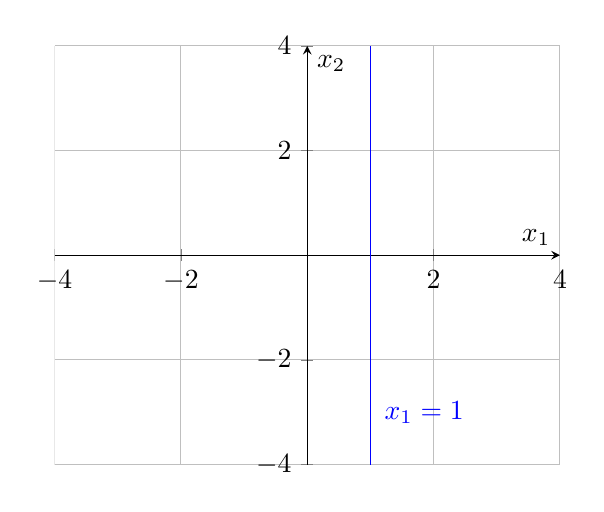
\begin{tikzpicture}
		\begin{axis}[
			axis lines=middle,
			xmin=-4, xmax=4,
			ymin=-4, ymax=4,
			grid=major,
			clip=false,
			xlabel=$x_1$, ylabel=$x_2$,
			]
			\addplot +[color=blue, mark=none] coordinates {(1, -4) (1, 4)}
			node at (axis cs:1.85,-3) {$x_1 = 1$};
		\end{axis}
	\end{tikzpicture}
\end{figure}

\subsection*{Question 1.4}

Given that $\theta = \begin{bmatrix}-64 & 0 & 0 & 1 & 1\end{bmatrix}^T$, we have:

\begin{equation*}
	y = \begin{cases}
		1, \quad &\text{if} \, ~ -64 + x_1^2 + x_2^2 \geq 0; \\
		0, \quad &\text{if} \, ~ -64 + x_1^2 + x_2^2 < 0 \\
	\end{cases}	
\end{equation*}

We can rearrange the inequalities to obtain our decision boundary as:

\begin{equation*}
	y = \begin{cases}
		1, \quad &\text{if} \, ~ x_1^2 + x_2^2 \geq 64; \\
		0, \quad &\text{if} \, ~ x_1^2 + x_2^2 < 64 \\
	\end{cases}	
\end{equation*}

Graphically, we can visualize the decision boundary as such:

\begin{figure}[!h]
	\centering
	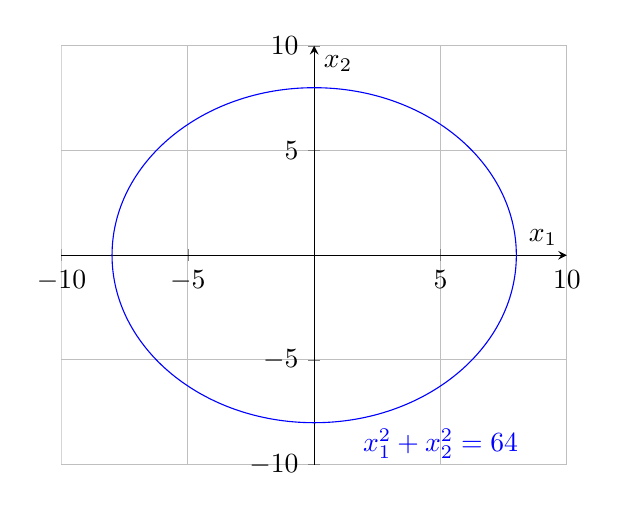
\begin{tikzpicture}
		\begin{axis}[
			axis lines=middle,
			xmin=-10, xmax=10,
			ymin=-10, ymax=10,
			grid=major,
			clip=false,
			xlabel=$x_1$, ylabel=$x_2$,
			]
			\draw [blue, radius=8] (axis cs:0,0) circle
			node at (axis cs:5,-9) {$x_1^2 + x_2^2 = 64$};
		\end{axis}
	\end{tikzpicture}
\end{figure}

\subsection*{Question 1.5}

Computers use finite binary bits to represent any number. As such, when computers need to represent real numbers, they perform floating-point arithmetic, which involves some form of approximation, as well as a trade off between precision and range. By progressively multiplying many probability values together as specified by Equation 1, most of which (if not all) are not whole numbers, computer machines will quickly give us a result that is too small to be meaningfully representable in computer memory. This is because probability values range between 0 and 1 inclusive, and as such, tend to be smaller (i.e., approach but do not equal zero) when multiplied together. This is also known as an underflow problem. In contrast, by following Equation 2, we can perform a computational sum over the terms that makes this problem less likely (although not impossible) to occur.

\end{document}
